\documentclass[color=blue, thmcnt=section, 12pt]{elegantbook}

% Title and author
\title{Machine Learning}
\author{Isaac FEI}

\cover{cover}

\begin{document}

% Print title and cover page
\maketitle

% Print table of contents
\frontmatter
\tableofcontents
\mainmatter

%------------------------------
% Main document starts from here
%------------------------------



%==============================
%==============================

\part{Elementary Concepts}

%==============================
%==============================






\chapter{Singular Value Decomposition (SVD)}

%------------------------------

\section{Theory}

%------------------------------

\begin{theorem}
    Let $A$ be an $m \times n$ real matrix with rank $r$. Then $A$ can be decomposed by 
    \begin{align*}
        A = U \Sigma V^\top
    \end{align*}
    where $U$ and $V$ are orthogonal matrices with shape $m \times m$ and $n \times n$, respectively. $\Sigma$ is an $m \times n$ matrix in the form of
    \begin{align*}
        \left[ \begin{array}{ccc|c}
            \sigma_1 &  & & \\ 
            & \ddots & & 0 \\ 
            & & \sigma_r & \\ 
            \hline
            & 0 & & 0
        \end{array} \right]
    \end{align*}
    where $\sigma_1, \ldots, \sigma_r$ are nonnegative numbers satisfying
    \begin{align*}
        \sigma_1 \geq \cdots \geq \sigma_r > 0
    \end{align*}
\end{theorem}

\begin{proof}
    % TODO
\end{proof}

%------------------------------

\section{Image Compression}

%------------------------------

\par Given a color image with height $m$ (pixels) and width $n$ (pixels), we first split the RGB channels. Then, each channel is regarded as an $m \times n$ matrix $A$. Applying the SVD to $A$, we obtain
\begin{align*}
    A = U \Sigma V^\top
\end{align*}
In practice, $A$ is very likely to have full rank, which means it has as many singular values as possible (at most $\min\left\{m, n\right\}$ singular values). But not all singular values along with its associated left and right singular vectors are of the same importance to the image, which we will explain in the following way.

\par For a pixel $a_{ij}$ located at the $i$-th row and $j$-th column in the image $A$, its value equals to 
\begin{align*}
    a_{ij} = \sum_{k=1}^n \sigma_k u_{ik} v_{jk}
\end{align*}
If the singular value $\sigma_k$ becomes very small starting from $k \geq r+1$, then the sum $\sum_{k=r+1}^n \sigma_k u_{ik} v_{jk}$ has little contribution to the pixel value $a_{ij}$. Hence, $a_{ij}$ can be approximated by 
\begin{align*}
    a_{ij} \approx \sum_{k=1}^r \sigma_k u_{ik} v_{jk}
\end{align*}

\par In this way, the original image $A$ can be compressed by only keeping the first $r$ singular values while dropping the rest. Mathematically, the compressed image $\hat{A}$ is given by
\begin{align*}
    \hat{A} = \hat{U} \hat{\Sigma} \hat{V}^\top
    = \begin{bmatrix}
        \mathbf{u}_1 & \cdots & \mathbf{u}_r
    \end{bmatrix} \begin{bmatrix}
        \sigma_1 & & \\ 
        & \ddots & \\ 
        & & \sigma_r
    \end{bmatrix} \begin{bmatrix}
        \mathbf{v}^\top_1 \\ \vdots \\ \mathbf{v}^\top_r
    \end{bmatrix}
\end{align*}
Recall $A$ represents a single channel. The final compressed color image can be then generated by merging all three compressed images from each channel.

\par We now demonstrate the algorithm to compress the image shown in Figure~\ref{fig:1}.
\begin{figure}[h!]
    \centering
    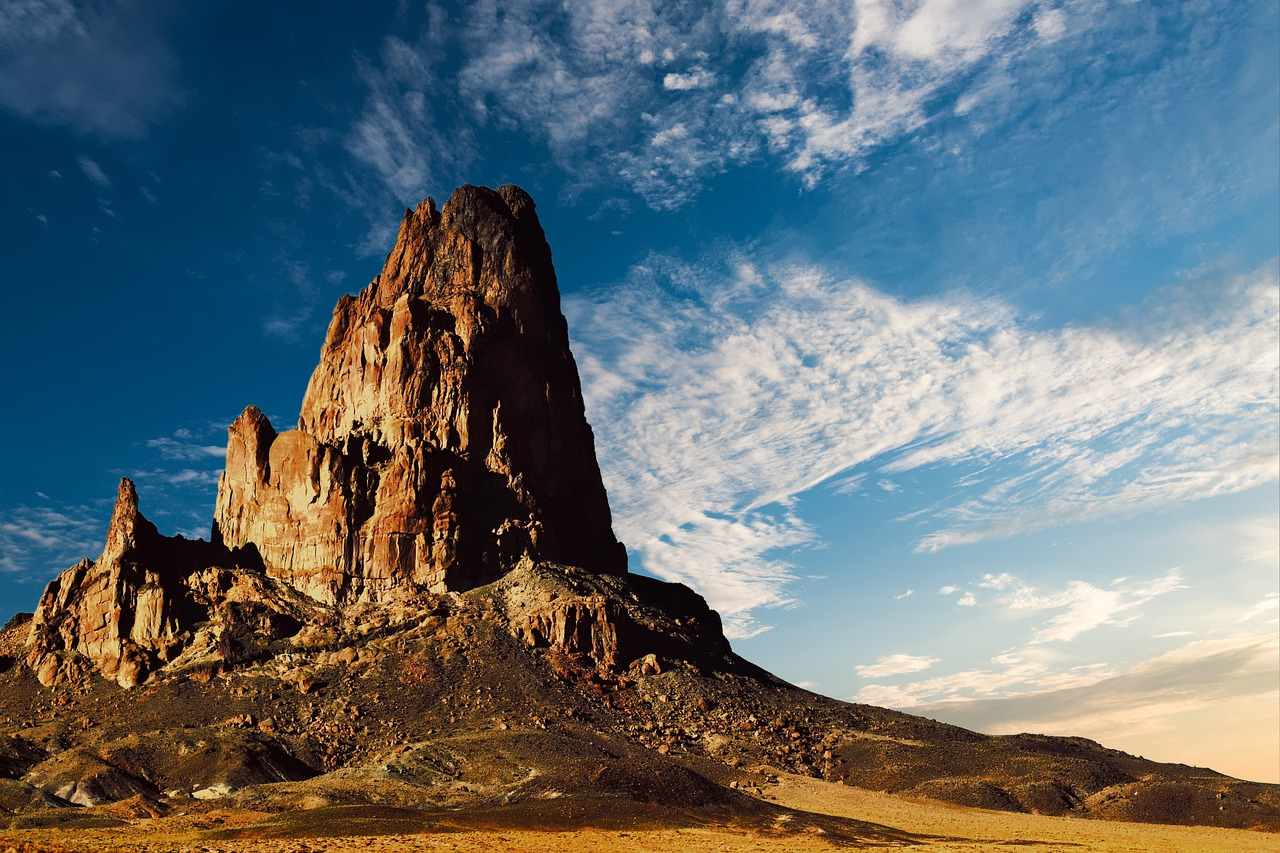
\includegraphics[scale=0.1]{figures/mountain.jpg}
    \caption{Mountain}
    \label{fig:1}
\end{figure}

%------------------------------

\section{Optimal Hard Threshold for Singular Values}

\par In practice, the approximate hard threshold for a \textit{square} matrix is given by 
\begin{align*}
    \tau \approx 2.858 \sigma_{\text{med}}
\end{align*} 

%==============================

\chapter{Principal Component Analysis (PCA)}

%------------------------------

\section{Maximizing a Quadratic Form}

\par In this section, we turn the focus maximizing a quadratic form $\mathbf{x}^\top A \mathbf{x}$ where $A \in \R^{n \times n}$ is an $n \times n$ positive semi-definite real matrix. To be concise, we shall adopt this setting of $A$ throughout this section. As we will see in a later section, this optimization problem plays an important role on the formulation of PCA.

\par Since $A$ is positive semi-definite, all its eigenvalues are nonnegative. By convention, we sort the eigenvalues in the descending order:
\begin{align*}
    \lambda_1 \geq \lambda_2 \geq \cdots \geq \lambda_n \geq 0
\end{align*}
And the corresponding eigenvectors are denoted by $\mathbf{v}_1, \ldots, \mathbf{v}_n$.

\begin{theorem} \label{thm:1}
    Consider the following optimization problem: 
    \begin{alignat*}{2}
        \max_{\mathbf{x}}&\quad & &\mathbf{x}^\top A \mathbf{x} \\ 
        \text{s.t.}& & &\norm{\mathbf{x}} = 1
    \end{alignat*}
    The solution to this problem is any normalized eigenvector $\mathbf{v}$ that is associated with the \textbf{largest} eigenvalue $\lambda_1$ of $A$. In particular, eigenvector $\mathbf{v}_1$ is a solution.
\end{theorem}

\begin{proof}
    % TODO
\end{proof}

%------------------------------

\begin{theorem} \label{thm:2}
    The solution to the optimization problem
    \begin{alignat*}{2}
        \max_{\mathbf{x}}&\quad & &\mathbf{x}^\top A \mathbf{x} \\ 
        \text{s.t.}& & &\begin{cases}
            \norm{\mathbf{x}} = 1\\ 
            \mathbf{v}_i^\top \mathbf{x} = 0
            \quad \forall 1 \leq i \leq j-1
        \end{cases}
    \end{alignat*}
    is any normalized eigenvector $\mathbf{v}$ associated with $\lambda_j$. In particular, eigenvector $\mathbf{v}_j$ is a solution.
\end{theorem}

\begin{proof}
    % TODO
\end{proof}

%------------------------------

\section{Maximizing the Variance}

%------------------------------

\par Let $(\mathbf{x}_1, \ldots, \mathbf{x}_n)$ be a sample of $d$-dimensional data with \textit{zero mean}, that is, $\mathbf{x}_i \in \R^d$ and $\bar{\mathbf{x}} = \mathbf{0}$. If the data does not have zero mean, then we can always first shift it so that it is centered at its mean. 

\par Now, we want to find a direction $\mathbf{w} \in \R^d$ ($\norm{\mathbf{w}} = 1$) such that all the data points projected to this direction will preserve the maximum variance. For point $\mathbf{x}_i$, let 
\begin{align*}
    t_i = \mathbf{w}^\top \mathbf{x}_i
\end{align*}
then our goal is to maximize $\var(t_1, \ldots, t_n)$, i.e., to solve the following optimization problem:
\begin{alignat*}{2}
    \max&\quad & &\var(t_1, \ldots, t_n) \\ 
    \text{s.t.}& & &\norm{\mathbf{w}} = 1
\end{alignat*}

\par It can be shown that 
\begin{align*}
    \var(t_1, \ldots, t_n)
    = \frac{1}{n-1} \sum_{i=1}^n \mathbf{w}^\top \mathbf{x}_i \mathbf{x}_i^\top \mathbf{w}
    = \mathbf{w}^\top S \mathbf{w}
\end{align*}
By Theorem~\ref{thm:1}, the maximum value of the variance $\var(t_1, \ldots, t_n)$ is the largest eigenvalue of the sample covariance matrix $S$.

\par What will happen if we apply the PCA to the sample data without first center it at its mean?

\begin{align*}
    \mathbf{w}^\top (\mathbf{x}_i - \bar{\mathbf{x}})
    = \mathbf{w}^\top \mathbf{x}_i 
    - \mathbf{w}^\top \bar{\mathbf{x}}
\end{align*}
This implies projected value or the component score will be shifted by $\mathbf{w}^\top \bar{\mathbf{x}}$. We can fix this by re-center it after PCA.

%------------------------------

\section{Minimizing the Reconstruction Error}

%------------------------------

\par Along a certain direction $\mathbf{w}$ ($\mathbf{w} = 1$), the projected point of $\mathbf{x}_i$ is given by (the data is assumed to have zero mean)
\begin{align*}
    \mathbf{p}_i = (\mathbf{w}^\top \mathbf{x}_i) \mathbf{w}_i
\end{align*}
Consider minimizing the mean square:
\begin{align}
    \frac{1}{n} \sum_{i=1}^n \norm{\mathbf{x}_i - \mathbf{p}_i}
    \label{eq:1}
\end{align}

\par Let $t_i = \mathbf{w}^\top \mathbf{x}_i$, it can be shown that 
\begin{align*}
    \frac{1}{n} \sum_{i=1}^n \norm{\mathbf{x}_i - \mathbf{p}_i}
    = \frac{1}{n} \sum_{i=1}^n \norm{\mathbf{x}_i}^2
    - \frac{n-1}{n} \var(t_1, \ldots, t_n)
\end{align*}
Therefore, to minimize the mean square error \eqref{eq:1} is equivalent to maximize the variance
\begin{align*}
    \var(t_1, \ldots, t_n)
\end{align*}

%------------------------------

\section{Probabilistic PCA (PPCA)}

%------------------------------

\par Suppose $(\mathbf{x}_1, \ldots, \mathbf{x}_n)$ is a sample of $d$-dimensional data. We assume random variable $\mathbf{x}$ is generated from some low dimensional latent variable $\mathbf{z} \in \R^l$ where typically $l \ll d$. Then $\mathbf{x}$ can be modelled by 
\begin{align*}
    \mathbf{x} = F \mathbf{z} + \boldsymbol{\mu} + \boldsymbol{\varepsilon}
\end{align*}
where $\boldsymbol{\mu}$ is the mean of $\mathbf{x}$ and $\boldsymbol{\varepsilon} \sim \mathcal{N}(\mathbf{0}, \sigma^2 I)$ is a noise term which captures the details of $\mathbf{x}$. The latent variable $\mathbf{z}$ is also assumed normal, more precisely, standard normal. That is, $\mathbf{z} \sim \mathcal{N}(\mathbf{0}, I)$. The parameters to fit are $F$, $\boldsymbol{\mu}$ and $\sigma^2$.

\par How to fit the parameters?

\par Optimal $F$:
\begin{align*}
    \hat{F} = U_l \left( \Lambda_l - \sigma^2 I \right)^{\frac{1}{2}} R
\end{align*}


\par Optimal $\sigma^2$:
\begin{align*}
    \hat{\sigma}^2 = \frac{1}{d - l} \sum_{i=l+1}^k \lambda_i
\end{align*}

%==============================

    
\end{document}